% Name: Diverging lens
% Description: Three parallel rays passing through a concave lens and spreading out, as if they came from the virtual focus F in front of it.
% Tags: concave lens, diverging lens, virtual focus, ray optics

\usepackage{optikz}
\usetikzlibrary{arrows.meta}

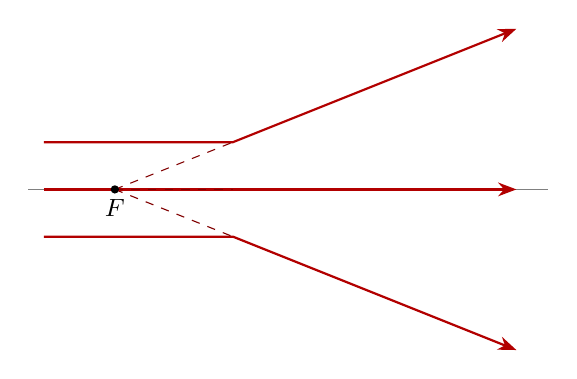
\begin{tikzpicture}[every node/.style={font=\small}]
  % Focal length 1.5: after the lens each ray at height h heads away from F = (-1.5, 0) along the line through F and (0, h)
  \draw[gray, thin] (-2.6,0) -- (4,0);
  \foreach \h in {-0.6, 0, 0.6} {
    \draw[thick, red!70!black, -{Stealth}] (-2.4,\h) -- (0,\h) -- ({3.6}, {\h*(1 + 3.6/1.5)});
    \draw[thin, dashed, red!50!black] (-1.5,0) -- (0,\h);
  }
  \concavelens[angle=0, width=0.5] at (0,0);
  \fill (-1.5,0) circle (1.5pt) node[below] {$F$};
\end{tikzpicture}
